\documentclass[10pt]{beamer}
\usepackage{uglixbeamer}
\title{Arborescences}
\subtitle{Chapitre 17}
\author{NSI2}

\begin{document}

\maketitle

\begin{frame}{Définition}
On appelle \alert{arborescence} un ensemble \textit{non vide} de n\oe uds tel que
\begin{enumerate}[--]
	\item 	un de ces n\oe uds est appelé \alert{racine} de l'arborescence;
	\item 	les autres n\oe uds sont partagés en $n$ sous-ensembles distincts qui sont eux-mêmes des arborescences;
    \item 	la racine est reliée aux $n$ racines de ces arborescences, qu'on appelle ses \alert{fils}.
\end{enumerate}
\begin{center}
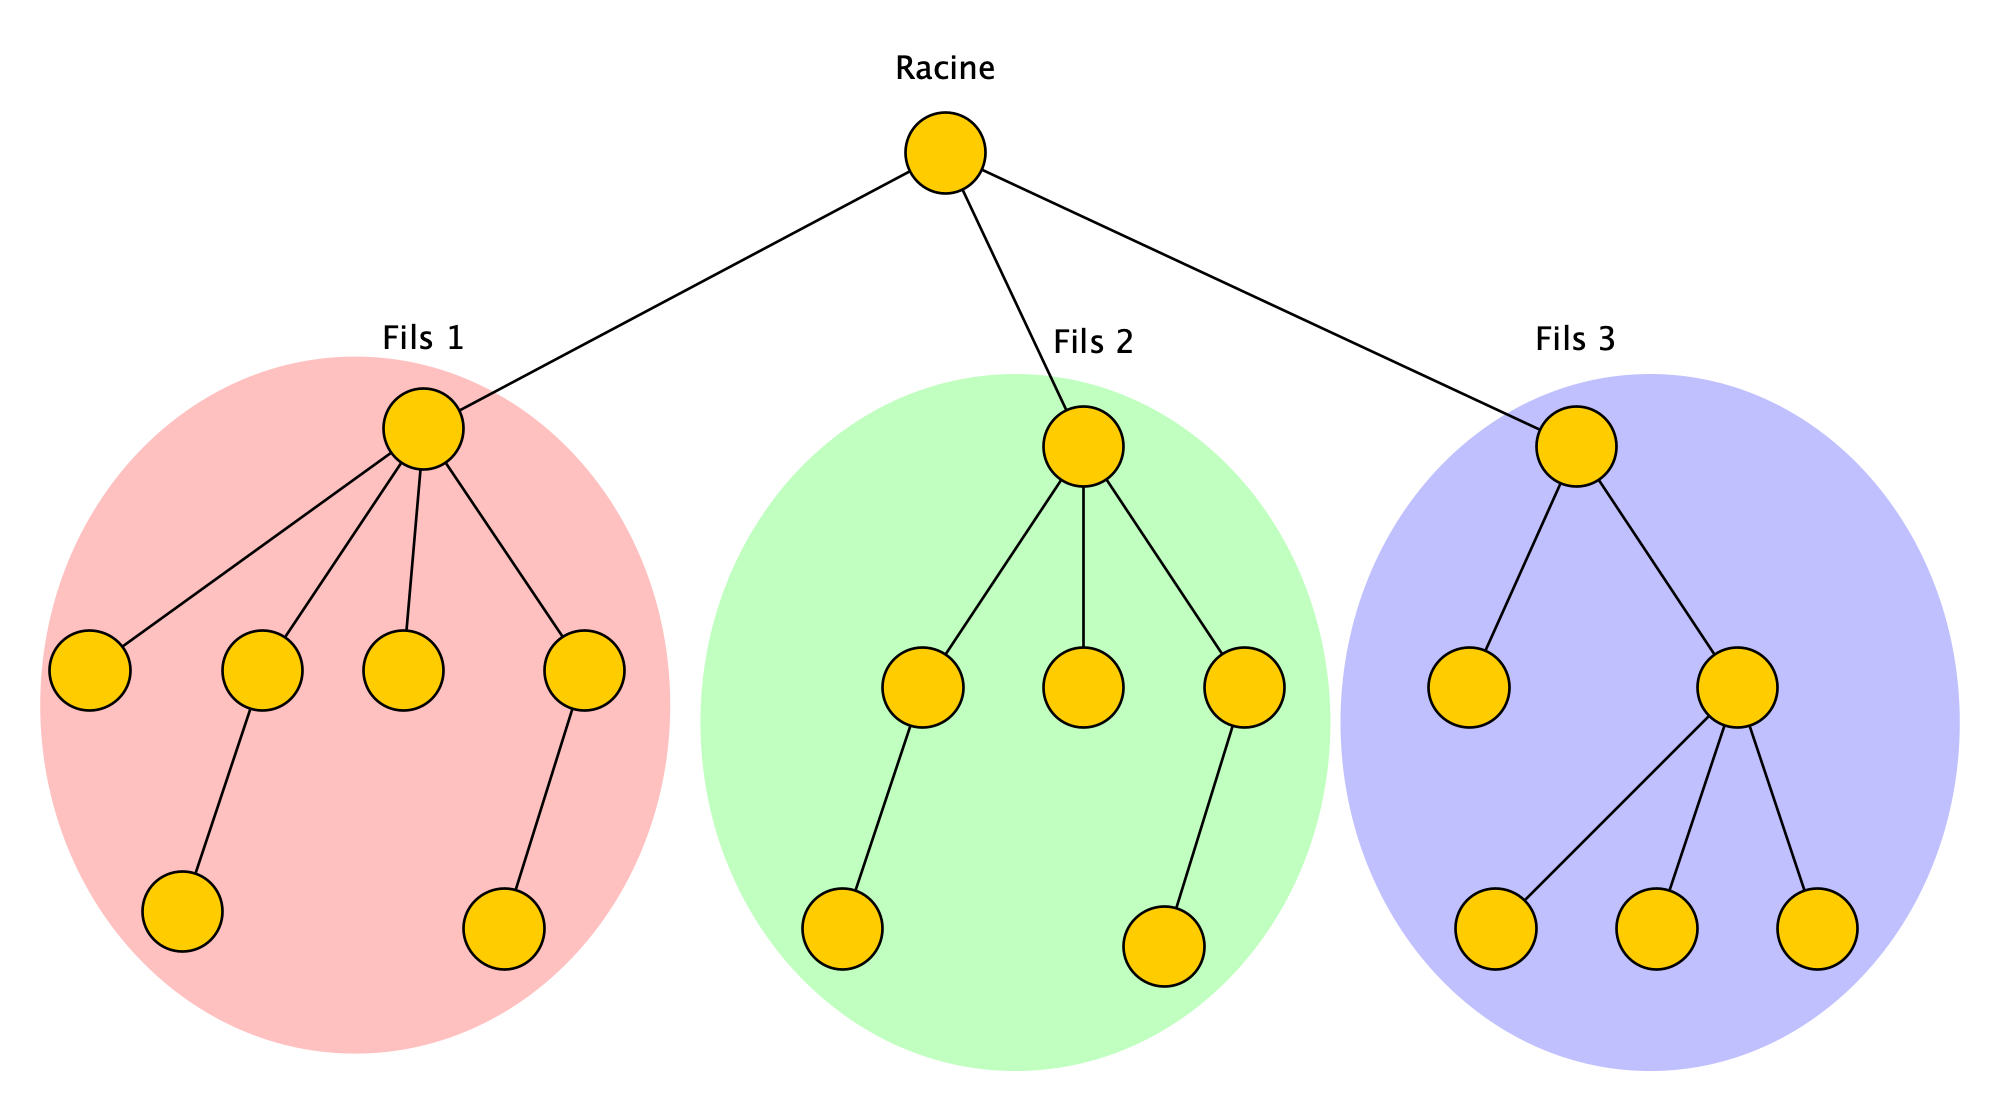
\includegraphics[width=8cm]{img/arbo1}
\end{center}
\end{frame}
\begin{frame}{Généralisation des arbres binaires ?}
Non :
\begin{enumerate}[--]
	\item 	il n'y a pas d'arborescence vide tandis que l'arbre binaire vide existe;
    \item 	dans un arbre binaire, il y a un ordre sur les fils (le gauche et le droit), dans une arborescence, il n'y a pas d'ordre sur les fils.
\end{enumerate}
Si le concept d'arborescence ne généralise pas celui d'arbre, il y a tout de même beaucoup de points communs.
\end{frame}
\begin{frame}{Taille et hauteur}
Les définitions sont les mêmes que pour les arbres binaires :
\begin{enumerate}[--]
	\item 	la \alert{taille} d'une arborescence est le nombre de ses n\oe uds;
	\item 	la \alert{hauteur d'un n\oe ud} est le nombre d'arêtes le reliant à la racine;
    \item 	la \alert{hauteur d'une arborescence} est la plus grande des hauteurs de ses n\oe uds.
\end{enumerate}
\begin{center}
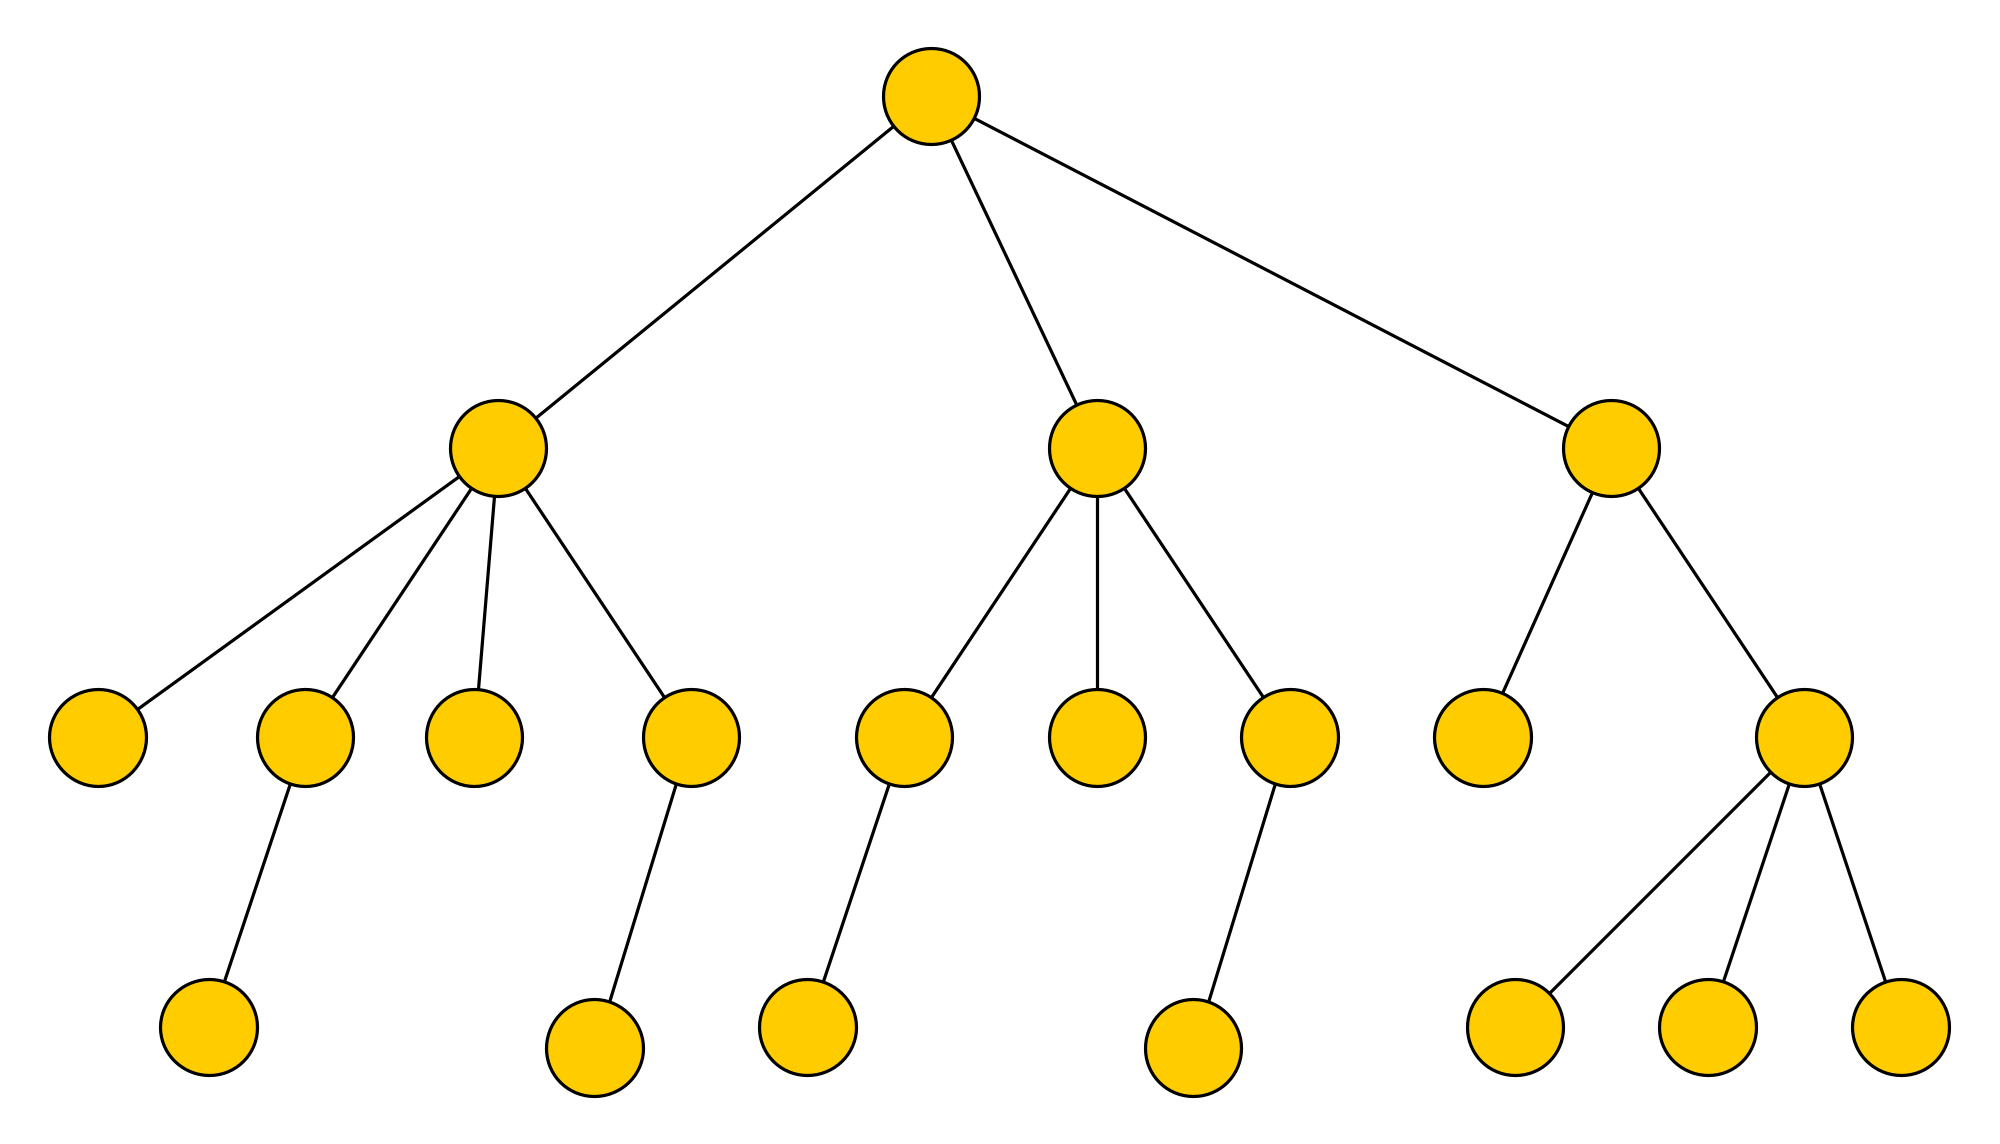
\includegraphics[width=6cm]{img/arbo2}\\
\textit{Arbre de taille 20 et de hauteur 3.}
\end{center}
\end{frame}
\begin{frame}[fragile]{Une implémentation possible}
\begin{minted}{python}
class NodeTS:
    def __init__(self, value):
        self.value = value
        self.children = []
\end{minted}

Un n\oe ud est une instance de la classe \pythoninline{NodeTS} (TS pour \textit{Tree Structure}, arborescence en Anglais).\\
Il possède un attribut \pythoninline{value} pour stocker une donnée, et un attribut \pythoninline{children} pour stocker la liste de ses fils, eux-mêmes instances de la classe \pythoninline{NodeTS}.
\end{frame}

\begin{frame}{Parcours d'une arborescence}
On retrouve la notion de parcours préfixe : 
\begin{enumerate}[--]
	\item 	traiter d'abord le n\oe ud courant;
	\item 	traiter ensuite les fils du n\oe ud (peu importe l'ordre).
\end{enumerate}
On retrouve également la notion de parcours postfixe :
\begin{enumerate}[--]
	\item 	traiter d'abord les fils du n\oe ud (peu importe l'ordre);
	\item 	traiter ensuite le n\oe ud courant.
\end{enumerate}
Il n'y a pas de parcours infixe.
\end{frame}
\begin{frame}{Exemples d'arborescences}
Le système de fichiers d'un lecteur logique \textsc{Windows} est une arborescence :
\begin{enumerate}[--]
	\item 	la racine est... la racine du lecteur : \texttt{C:} par exemple
	\item 	chaque n\oe ud est un dossier contenant un ensemble de fichiers, et avec des dossiers fils.	
\end{enumerate}
\end{frame}
\begin{frame}{En biologie}
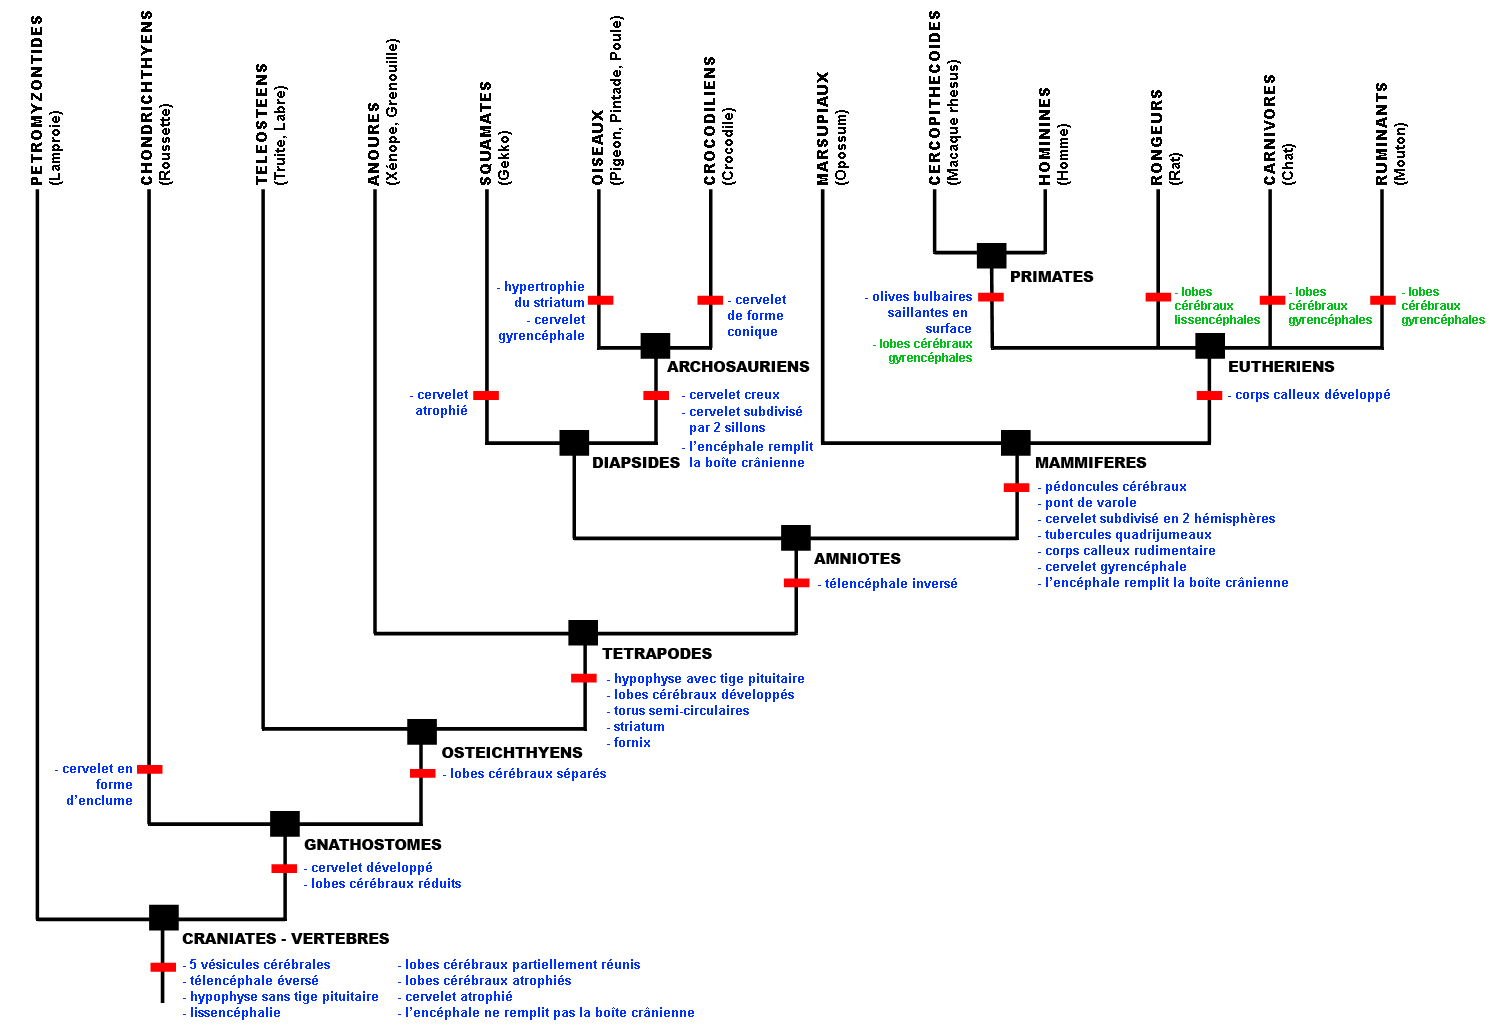
\includegraphics[width=\linewidth]{img/philo}
\end{frame}
\begin{frame}[fragile]{Langage XML}
\inputminted[fontsize=\small]{xml}{scripts/recette.xml}
\end{frame}
\begin{frame}{Langage XML}
C'est un langage à balises pour décrire des données structurées :
\begin{enumerate}[--]
	\item 	une recette, comme dans l'exemple précédent;
	\item 	la valeur des attributs d'un objet...
\end{enumerate}
Un document XML est une arborescence. Toute portion \textit{complète du code}, c'est-à dire :
\begin{enumerate}[--]
	\item 	une portion commençant par une balise et terminant par la balise fermante correspondante, correspond à un n\oe ud;
	\item 	une portion sans balises.
\end{enumerate} 
\end{frame}
\begin{frame}{Trie}
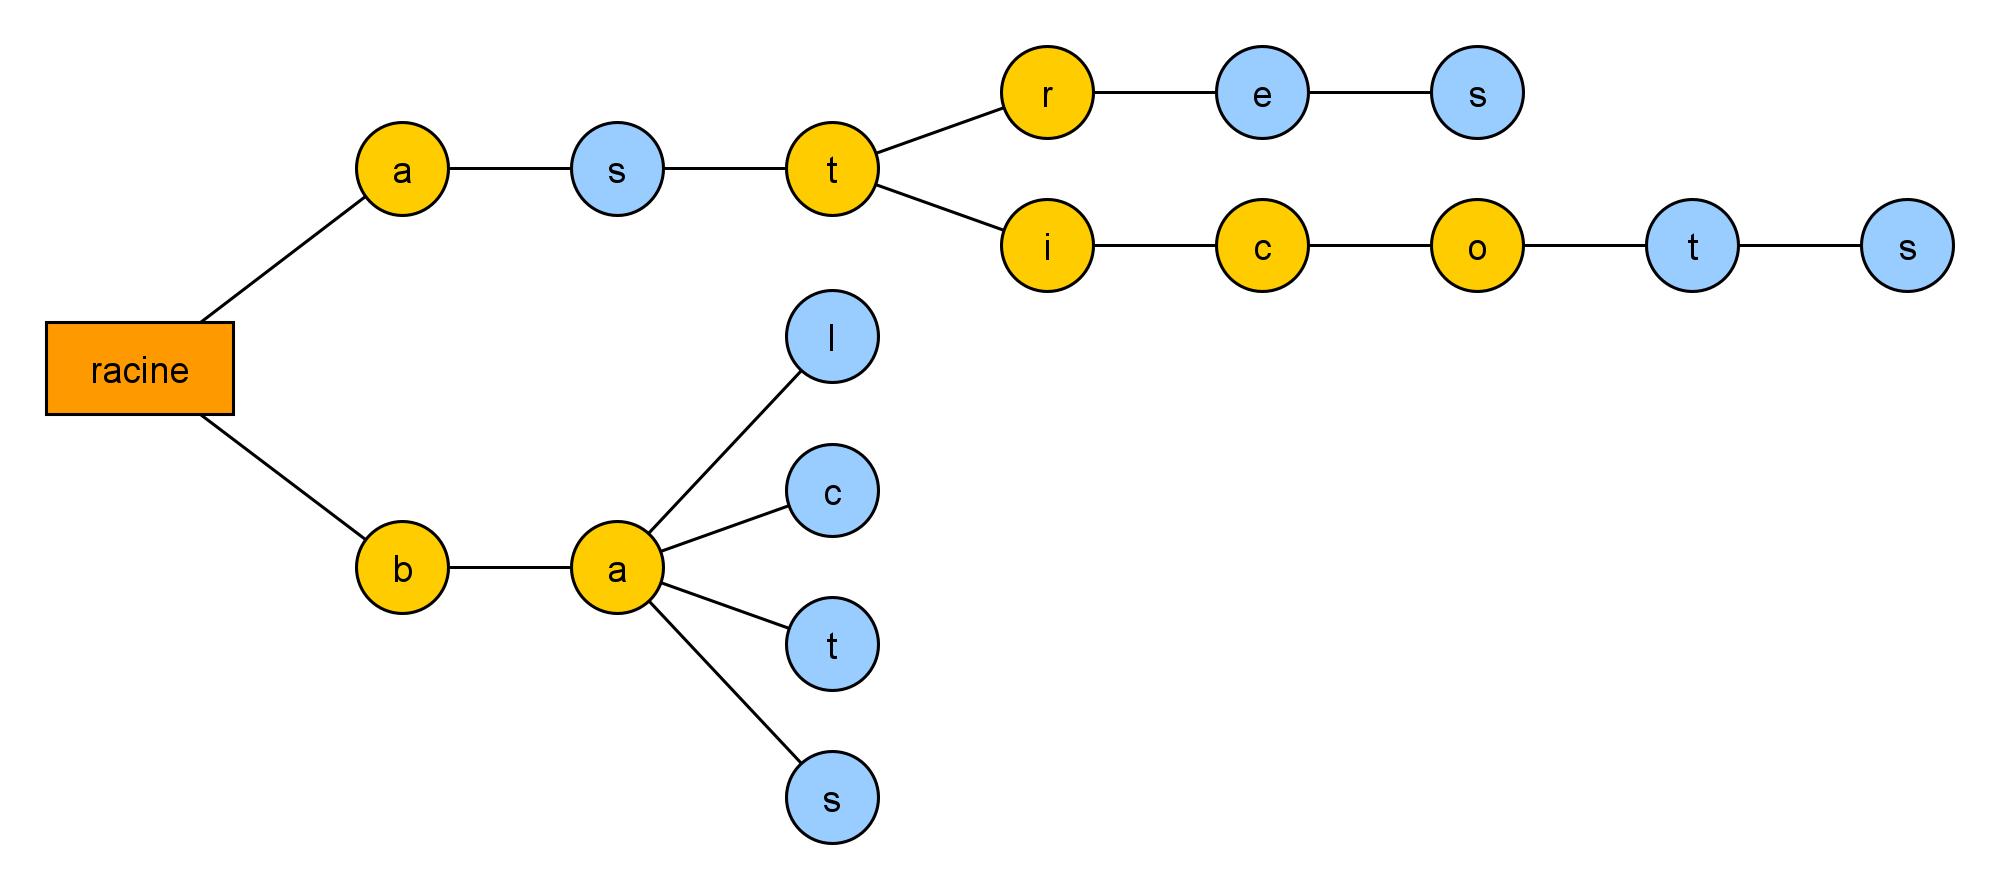
\includegraphics[width=\linewidth]{img/trie}
On part d'une racine \og vide\fg{}. Chaque n\oe ud contient une lettre et un booléen indiquant si cette lettre est la fin d'un mot ou non.\\
Ici le trie contient les mots as, astre, astres, asticot, asticots, bal, bac, bat et bas.
\end{frame}
\begin{frame}{Implémentation d'un trie}
Elle diffère légèrement de celle d'une arborescence traditionnelle.\\

Nous verrons cela en exercice.
\end{frame}
\end{document}